% Time-stamp: Sun Jul 28 14:00:00 2013
% !TEX root =  free234.tex
\chapter{Functions of more than one variable} 

\section{Functions of two variables and their graphs} 
\subsection{Definition} 
A function of two variables has two ingredients: a \textit{domain} and \textit{a
rule}.  The domain of the function is a collection of points in the $xy$-plane.
For each point $(x,y)$ from the domain of the function, the rule
should tell us how to find the function value $f(x,y)$.

Just as with functions of one variable, the ``rule'' that gives us the function
value is often specified by some formula, e.g.~$f(x,y) = x+y$.  The domain of a
function is the set of points at which we define the function.  This can in
principle be any set of points in the plane.  Typically the domain will be a
rectangle, or a disc, or it could be the entire $xy$-plane, possibly with some
points and lines removed.

\begin{figure}[h]
  \begin{center}
    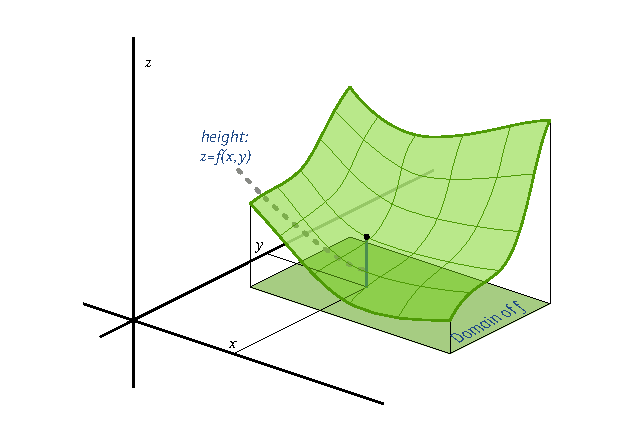
\includegraphics{01Agraph.pdf}
  \end{center}
  \caption{The graph of some function, and its domain (a rectangle in this
  example).}
  \label{fig:01Agraph}
\end{figure}

\subsection{Graphs} By definition, the graph of a function 
$z=f(x,y)$ is the collection of all points $(x,y,z)$ in three dimensional space
that satisfy the equation $z=f(x,y)$.

The graph is usually a surface that floats above (or below) the domain of the
function (see Figure~\ref{fig:01Agraph}).

\subsection{Level sets}  The graph of a function of two variables 
is a surface sitting in three dimensional space, which can be difficult to draw
or visualize.  Instead of looking at the graph we can also consider its level
sets.  If $c$ is any real number, then, by definition, the \emph{level set at
level $c$} of the function is the set of all points $(x,y)$ in the plane that
satisfy $f(x,y) = c$.

\begin{figure}[h]
  \begin{center}
    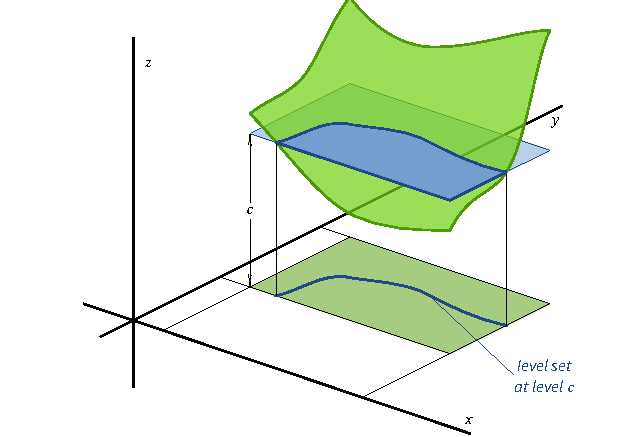
\includegraphics{01Agraphwithlevelsets.pdf}

    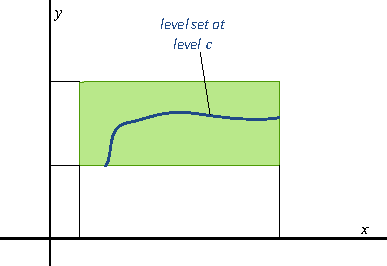
\includegraphics{01levelsets-without-the-graph.pdf}
  \end{center}
  \caption{The graph of some function (\textit{top}), and a construction of one
  of its level sets (\textit{bottom}).  Note that \textit{by definition} the
  level set (``at level $c$'') is the curve in the $xy$-plane under the graph:
  it is obtained by intersecting the graph of the function with a horizontal
  plane at height $c$, and then projecting this curve of intersection onto the
  $xy$-plane.  }
  \label{fig:01Agraph}
\end{figure}

Since the level set is the set of all solutions to the equation $f(x,y)=c$, one
often uses the notation $f^{-1}(c)$ (``$f$-inverse of $c$'') for the level set.
We can summarize the definition in an equation:
\[
  f^{-1}(c)
  =
  \bigl\{ (x,y) : f(x,y) = c\bigr\}.
\]%
\marginwarning%
Note that the definition says that $f^{-1}(c)$ \emph{is not a number, but a set
of points!}

Level sets tend to be curves in the $xy$-plane, although in general level sets
can have any shape (see Problem~\ref{prb:distance-to-square-level-sets} for an
example.)  They are usually easier to draw than the graphs of the corresponding
functions.

\subsection{An example from the ``real'' world} 
\label{sec:01mendotaexample}  Here is a function of local interest.  The domain
of the function is the water surface of Lake Mendota (let's pretend this is a
plane domain), and the function, which we will call $d$ instead of $f$, is given
by $d(x, y) = $ the depth of the lake at location $(x, y)$.  There is no formula
for this function, but the Wisconsin Department of Natural Resources has
measured the depth and presented the results in terms of the level sets of the
function $d$.


\begin{figure}[ht]
  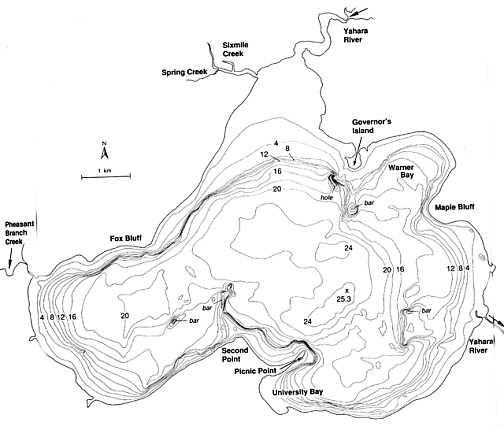
\includegraphics[width=0.70\textwidth]{01Mendota.jpeg}
  \caption{  The level curves of a function $z=d(x, y)$.  The domain of this
  function is the lake surface, and $d(x, y)$ is the depth in meters of Lake
  Mendota at $(x, y)$.  To see the graph of the function we could try to drain the
  lake.\\
  \null\quad%
  See \url{http://limnology.wisc.edu/lake_information/mendota/mendota.html} }
\end{figure}

\subsection{A comment about language and set-theoretic notation} 
We will often say ``consider a function $z=f(x,y)$\dots'', but there is a
sense in which this is incorrect.  It is convenient to say ``consider a function
$z=f(x,y)$\dots'' since it not only names the function, but it also gives the
independent variables $x$, $y$, and the dependent variable $z$ a name.
Nevertheless, the symbol in the equation $z=f(x,y)$ that actually represents the
function is ``$f$''.  The correct way of introducing the function\footnote{%
Saying ``consider the function $z=f(x,y)$\dots'' to introduce the function $f$ is
like saying ``Please meet my brother Joe, Bill, and Sue'' when you want to
introduce your brother Joe, who happens to be standing next to Bill and Sue.  To
introduce your brother, you would of course say ``Please meet my brother
Joe.'' and to introduce the function you should really say ``Consider the
function $f$.''}
would be to say ``consider a function $f$.''

In fact, in the notation that is used in modern mathematics one would write
``Consider the function $f:D\to\R$\dots''  Here $f$ is the name of the function
we are introducing, $D$ is the domain of that function (so $D$ is a set of
points in the plane), and $\R$ stands for the set of real numbers, indicating
that computing $f$ always results in a real number.

\subsection{Vector notation} If $\vx$ is the position vector 
of the point $(x, y)$ in the plane, i.e.\ if $\vx = \tvek x\\ y\ttor$, then one
sometimes writes
\[
f(x, y)  = f(\vx).
\]
Physicists have a preference for $\vr$ instead of $\vx$ (because they call the
position vector the ``radius vector''), and will write $f(x,y) = f(\vr)$.



\section{Linear functions} 
The simplest function of one variable are those of the form $f(x) = ax+b$.
Their graphs are lines, and we called them linear functions.

A linear function of two variables is a function $f$ of the form
\begin{equation}
  z=f(x,y) = ax+by+c,
  \label{eq:linear-function}
\end{equation}
where $a,b,c$ are constants.

\begin{figure}[h]
  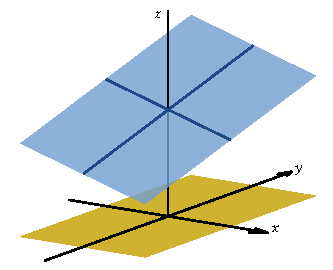
\includegraphics{01graph-of-a-linear-function.pdf}
  \caption{The graph of a linear function $z=ax+by+c$. }
  \label{fig:graph-of-lin-f}
\end{figure}
The graph of a linear function is always a plane.  Indeed, the graph consists of
all points $(x,y,z)$ that satisfy the equation
\[
  -ax-by+z = c,
\]
which we can write as 
\[
  \vn\dpp\vx = \vn\dpp\vp,
\]
where
\[
  \vn = \vek -a\\ -b\\ 1\tor, \quad \text{and}\quad
  \vp = \vek 0 \\ 0 \\ c\tor.
\]

\section{Quadratic forms} 
\label{sec:quadratic-forms}%
After learning about linear functions in pre-calculus one usually goes on to
quadratic functions.  We will do the same for functions of two variables and
study \textit{Quadratic Forms}.  Just as in the one variable case where
quadratic functions can have a maximum or minimum, quadratic forms provide
examples of functions of two variables that can have a maximum or a minimum, or,
it turns out, a third kind of ``min-max'' or ``saddle shape.'' They provide the
basic profile of what we will run into when we look for local minima and maxima
of functions of two variables.  In particular, the technique of classifying
quadratic forms by completing the square, which we will see in this section, is
the key to the second derivative test for functions of more than one variable.


\subsection{Definition} 
The general quadratic form in two variables is
\begin{equation}
  f(x,y) = Ax^2 + Bxy + Cy^2,
  \label{eq:general-quadratic-form}
\end{equation}
where $A$, $B$, and $C$ are constants.  Depending on the values of these
constants the graphs of the functions can have a number of different shapes.

In addition to these quadratic forms one can also consider the more general
class of quadratic functions,
\[
  f(x,y) = Ax^2 + Bxy + Cy^2 + Dx + Ey + F,
\]
which also have terms of degree 1 and 0.
We will restrict ourselves to quadratic forms (for now).

\subsubsection*{The prototypical examples}

There are several important special cases that are representative of what the
graphs of quadratic forms can look like.  These special cases are
\begin{subequations}
  \begin{align}
    f(x,y) & = x^2+y^2, \text{ and } g(x,y) = -x^2-y^2,
    \label{eq:qform-definite}\\
    h(x,y) & = x^2, \text{ and } \tilde h(x,y) = -x^2,
    \label{eq:qform-semidefinite}\\
    k(x,y) & = xy
    \label{eq:qform-indefinite}
  \end{align}
\end{subequations}
Their graphs are discussed in Figure~\ref{fig:typical-q-forms}.
\begin{figure}[b]\flushleft
\color{darkbluegreen}\sffamily
\noindent%
\rule{\textwidth}{1pt}
\vglue2pt
\noindent%
\begin{minipage}{0.42\textwidth}
  The two forms $f$ and $g$ from \eqref{eq:qform-definite} are called
  \emph{\color{badgerred}definite}, since they cannot change sign:
  \[
    f(x,y) = x^2+y^2
  \]
  is the sum of two squares, and therefore is always positive, unless both $x$
  and $y$ vanish.  Similarly, $g(x,y) = -f(x,y)$ is always negative, except at
  $(x,y) = (0,0)$.
\end{minipage}\hfill
\parbox{0.55\textwidth}{
  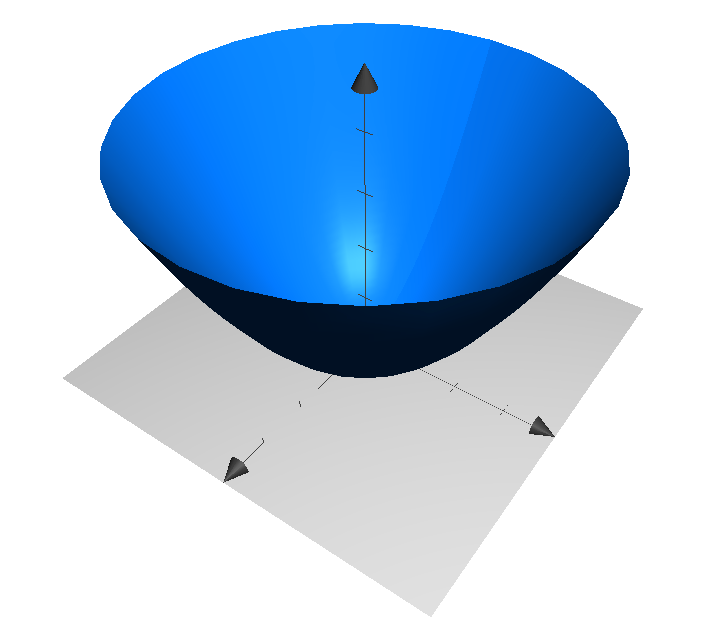
\includegraphics[width=0.25\textwidth]{01minimum.png}
  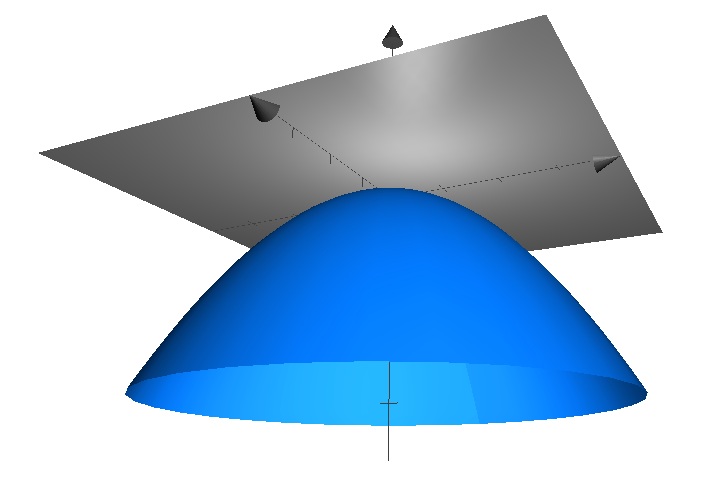
\includegraphics[width=0.25\textwidth]{01maximum.png}
  }


\noindent%
\rule[-0.5ex]{0pt}{1ex}%
\rule{\textwidth}{0.2pt}
\noindent%
\begin{minipage}{0.42\textwidth}
 The form $h(x,y) = x^2$ is called
  \emph{\color{badgerred}semidefinite} because it too cannot change its sign.
  Clearly, $h(x, y)=x^2$ is never negative, but for $h(x, y)$ to be positive, we
  need $x\neq0$.
  So, the function $h(x,y)$ is positive, except on the line $x=0$ (the $y$
  axis).  The graph of the function $\tilde h(x, y) = -y^2$ is similar, but
  upside down.
\end{minipage}
\parbox{0.55\textwidth}{
  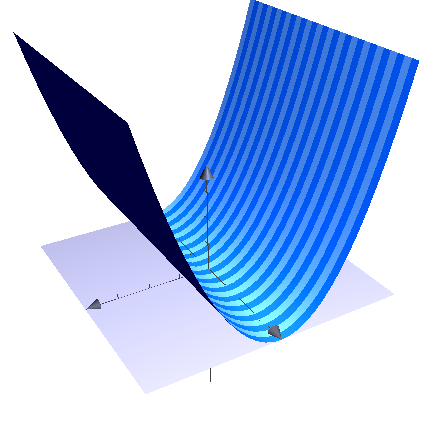
\includegraphics[width=0.25\textwidth]{01degenerate-minimum.png}
  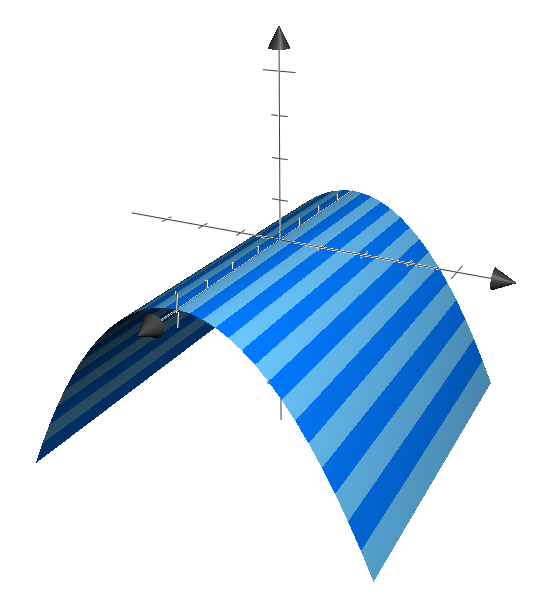
\includegraphics[width=0.25\textwidth]{01degenerate-maximum.png}
}


\noindent%
\rule[-0.5ex]{0pt}{1ex}%
\rule{\textwidth}{0.2pt}
\noindent%
\begin{minipage}{0.42\textwidth}
 The form $k(x, y) = xy$ is called \emph{\color{badgerred}{indefinite},} because
 it can be both positive and negative:  if $x$ and $y$ have the same sign, then
 $xy>0$, but if they have opposite signs, then $xy<0$.  Thus the graph of $z=xy$
 lies above the $xy$-plane in the first and third quadrants, and below the
 $xy$-plane in the second and fourth quadrants.
\end{minipage}
\parbox{0.55\textwidth}{%
\def\svgwidth{0.25\textwidth}
  \input ../figures/234/01saddle-signs.pdf_tex
  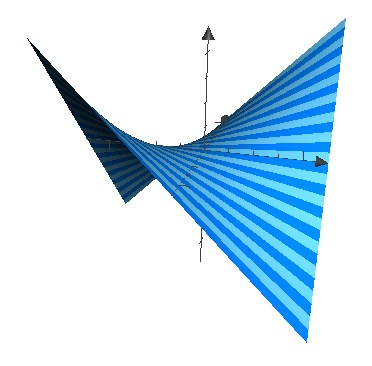
\includegraphics[width=0.25\textwidth]{01saddle-stripes.png}
  }

\noindent%
\rule{\textwidth}{1pt}
\caption{Graphs of some representative quadratic forms.}
\label{fig:typical-q-forms}
\end{figure}

\subsection{Classifying quadratic forms -- the general procedure} 
All quadratic forms have graphs that look like one of the examples shown above
-- but how can we tell which it is?  In other words, if $Q(x, y)$ is a given
quadratic form how can we tell if it is definite, indefinite, or semidefinite?
How do we know for which $(x, y)$ the form $Q(x, y)$ is positive or negative?
It turns out that we can always find out by using the trick of ``completing the
square.''

The general procedure for a given quadratic form $Q(x, y) = Ax^2+Bxy+Cy^2$ is as
follows:
\begin{enumerate}
\item If $A=0$, then we really have $Q = Bxy+Cy^2$ and we can factor $Q$ as
  \[
    Q(x, y) = (Bx+Cy)y.
  \]
\item Assume $A\ne 0$.
  We factor out $A$, and complete the square for the
  first two terms:
\begin{align*}
    Q(x, y) &= A\Bigl\{x^2+\frac{ B}{A}xy + \frac CA y^2\Bigr\}\\
    &=A \Bigl\{\bigl(x+\frac{B}{2A}y\bigr)^2 - \bigl(\frac{B}{2A}y\bigr)^2 + 
    \frac CA y^2\Bigr\}\\
    &=A \Bigl\{
    \underbrace{
      \bigl(x+\frac{B}{2A}y\bigr)^2
    }_{u^2}
    + \underbrace{
      \frac{\color{badgerred}4AC-B^2}{4A^2}y^2
    }_{\pm v^2}
    \Bigr\}.
\end{align*}
\item If $4AC-B^2>0$, then the expression in braces is positive, and we can
  write 
  \[
    Q(x, y) = A(u^2+v^2), \quad\text{where}\quad
    u = x+\frac{B}{2A}y, \text{ and }
    v = \frac{\sqrt{4AC-B^2}}{2A}y.
  \]
  Depending on the sign of $A$ our function is always positive or always
  negative, and we say the form is \emph{positive definite} or \emph{negative
  definite.}
\item If $4AC-B^2<0$, then we have
  \[
    Q(x, y) = A(u^2-v^2), \quad\text{where}\quad
    u = x+\frac{B}{2A}y, \text{ and }
    v = \frac{\sqrt{B^2-4AC}}{2A}y.
  \]
  When this happens we can factor the quadratic form, i.e.~we have
  \[
    Q(x, y) = A (u+v)(u-v).
  \]
  The form is \emph{indefinite.}
\item in the only remaining case we have $4AC-B^2=0$, so that
  \[
    Q(x, y) = A\Bigl(x+\frac{B}{2A}y\Bigr)^2.
  \]
  In this case the form is a perfect square (times $A$).
  The form is \emph{semi-definite.}

\end{enumerate}
To understand this procedure it is perhaps best to look at how it works in some
examples.

\subsection{Classifying quadratic forms -- two examples} 

\subsubsection{An indefinite quadratic form} 
\label{sec:quad-form-example-indefinite}
Consider the form $Q(x, y) = -3x^2+9xy+6y^2$. We rewrite this as
follows:
\begin{align*}
  Q&= -3x^2+6xy+9y^2\\
  &=-3\bigl(x^2 - 2xy -3y^2\bigr) \\
  &= -3\bigl[\underbrace{x^2  - 2xy + y^2}_{} -4 y^2\bigr]
  & \parbox{160pt}{\dfnt%
  complete the square}\\
  &= -3\bigl[(x-y)^2 - 4y^2\bigr]
  & \parbox{160pt}{\dfnt\raggedright%
   in this case we get the difference of two squares,
   so use $a^2-b^2 = (a-b)(a+b)$}\\
  &= -3(x-y-2y)(x-y+2y) \\
  &= -3(x-3y)(x+y).
\end{align*}
This shows that $Q(x, y) > 0$ when $y>\tfrac 13 x$ or $y<-x$,
and $Q(x, y) <0$ when $-x < y < \tfrac 13x$.

\begin{figure}[h]
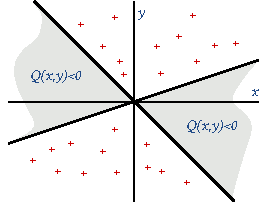
\includegraphics{03Q-signs.pdf}
\caption{The signs of the quadratic form in example
  \ref{sec:quad-form-example-indefinite}.}
\end{figure}

\subsubsection{A positive definite quadratic form}
\label{sec:quad-form-example-positive-definite}
To see a different example, consider the quadratic form $Q(x, y) = 2x^2-4xy+6y^2$.
By completing the square we can write it as
\begin{align*}
  Q(x, y)
  &= 2\, \bigl\{x^2 -2xy + 3y^2\bigr\} & \\
  &= 2\, \bigl\{\color{blue}x^2-2xy+y^2\color{black} + 2y^2\bigr\}
  &\parbox{160pt}{\dfnt the square is complete}\\
  &= 2\, \bigl\{\color{blue}(x-y)^2\color{black} + 2y^2\bigr\} &\\
  &= 2(x-y)^2 + 4y^2.
\end{align*}
We see that this particular quadratic form is positive definite.


\section{Functions in polar coordinates $r,\theta$} 
\label{sec:functions-in-PC}%
Recall that instead of using Cartesian coordinates $(x,y)$ to specify the location
points in the plane, we can also use polar coordinates.  In many cases it is much
easier to describe a function using polar coordinates than in Cartesian coordinates.

To go back and forth between Cartesian and Polar Coordinates we can use the following
relations
\begin{subequations}
  \begin{align}
    x &= r\cos\theta \\
    y &= r\sin\theta \\
    r &= \sqrt{x^2 + y^2} \\
    \text{\color{red}\carefulnow}\; \theta &= \arctan\frac{y}{x}\; 
    \text{\color{red}\carefulnow}
  \end{align}%
  \label{eq:PC-xy-relations}%
\end{subequations}%
The equation for $\theta$ is only valid for $x>0$, where $-\frac\pi2 < \theta <
\frac \pi2$.  In other regions of the plane there are other expressions relating
$\theta$ to $(x,y)$.  See problem~\ref{prb:polar-angle-formula}.

\begin{figure}[h]
  \flushleft%
  \parbox{0.45\textwidth}{
  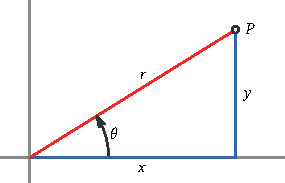
\includegraphics{01PC.pdf}
  }\hfill
  \parbox{0.45\textwidth}{
  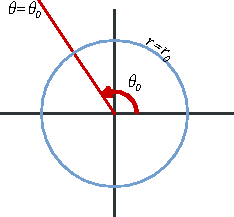
\includegraphics{01theta-r-constant.pdf}
  }
  \caption{Polar coordinates are defined in the picture on the right (see also
  equations \eqref{eq:PC-xy-relations}).  On the left:  the set of points at which
  $\theta$ has one given value $\theta_0$ form a half line emanating from the origin
  that makes an angle $ \theta_0$ with the positive $x$-axis.   The set of points at
  which $r$ has a given value $r_0$ form a circle centered at the origin, with radius
  $r_0$.}
\end{figure}

The simplest kinds of functions one can consider in polar coordinates are those that
only depend on one of those coordinates, i.e.~functions that only depend on the
radius $r$, and functions that only depend on the polar angle $\theta$.
Let's look at some examples of such functions.

\subsection{Radially symmetric functions} 
\label{sec:functions-in-PC-radial}%
The functions
\[
  f(x, y) = x^2+y^2, \quad
  g(x, y) = \sqrt{x^2+y^2}, \quad
  h(x, y) = \ln\bigl(x^2+y^2\bigr),
\]
all can be expressed in terms of the radius $r$ only.  Namely, using $r^2=x^2+y^2$, we
have
\[
  f(x, y) = r^2, \quad
  g(x, y) = r, \quad
  h(x, y) = \ln r^2 (= 2\ln r).
\]
In general, a function $z=f(x, y)$ that can be written in terms of the radius $r$
only, i.e. a function for which there is some function $\Phi$ of one variable with
\[
  f(x, y) = \Phi(r), \quad
  \text{i.e. } f(x, y) = \Phi\bigl(\sqrt{x^2+y^2}\bigr),
\]
is called a \emph{radially symmetric function.}  

Since a radially symmetric function only depends on the radius $r$, its level sets
consist of circles centered at the origin (one exception:  the origin, $r=0$ can
also be a level set, and this is obviously not a circle but a point.)

As an example, we consider the function $g(x, y) = \sqrt{x^2+y^2} = r$ in more detail.
The function $\Phi$ of one variable here is $\Phi(r) = r$.  We can try to visualize
the graph of $g$ by first looking at the positive $x$-axis only.  There we have $f(x,
0)=\sqrt{x^2} = x$.  We get the graph of $g$ by revolving the graph of $z=x$ around
the $z$-axis.  See Figure~\ref{fig:graph-of-z-is-r}.
\begin{figure}[t]
  \def\svgwidth{0.6\textwidth}%
  \input ../figures/234/01cone.pdf_tex
  \caption{\textbf{Radially symmetric functions.}  The graph of $z=r$.}
  \label{fig:graph-of-z-is-r}
\end{figure}

\subsection{Functions of $\theta$ only} 
\label{sec:functions-in-PC-theta}%
Here are two functions that happen to depend on the polar angle $\theta$ only:
\[
  f(x, y) = \sin\theta, \qquad h(x, y) = \theta.
\]
We can rewrite these functions in terms of $x$ and $y$ by using the relations between
Cartesian and Polar coordinates \eqref{eq:PC-xy-relations}.  We get
\[
  f(x, y) = \sin\theta = \frac{y}{r} = \frac{y}{\sqrt{x^2+y^2}}
\]
for $f$, and 
\[
  h(x,y) = \theta = \arctan \frac{y}{x}
\]
for $h$, at least in the right half plane where $x>0$. 

A function that only depends on $\theta$ is constant on rays emanating from the origin
because the polar angle $\theta$ is constant on such rays. The level sets of such
a function therefore consist of half-lines (``rays'') starting at the origin. Its
graph consists of ``spokes'' attached to the $z$-axis.  Each spoke lies above a ray
in the $xy$-plane with some polar angle $\theta$, and is attached to the $z$-axis at
a height given by the function value.  As we vary $\theta$, the spoke rotates around
the vertical axis and moves up or down, as dictated by the function.
Figure~\ref{fig:graph-of-f-of-theta} shows what happens for $f(x, y) = \sin\theta$.

\begin{figure}[h]
  \begin{minipage}{0.4\textwidth}
    \centering
    \dfnt 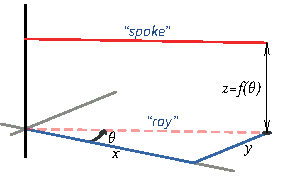
\includegraphics{01PC-graph-of-f-theta.pdf}\\
    The graph of a function of $\theta$ only consists of horizontal spokes attached to
    the $z$-axis.
  \end{minipage}
  \begin{minipage}{0.55\textwidth}
    \centering
    \dfnt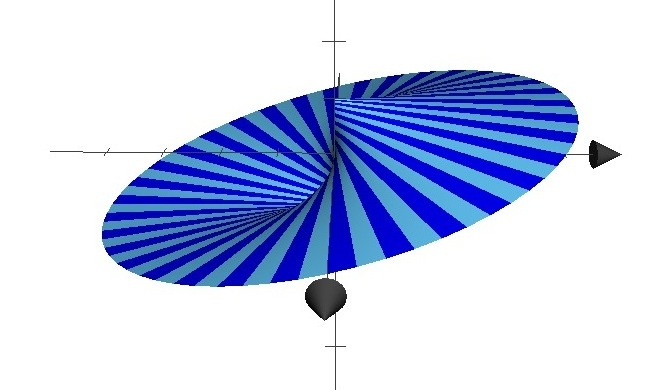
\includegraphics[width=0.95\textwidth]{01function-of-theta.jpeg}\\
    The graph of $z=\sin\theta$\\
    (the $x$-axis is coming right at us.)
  \end{minipage}
  \caption{}
  \label{fig:graph-of-f-of-theta}
\end{figure}

The function $z=\theta$ has a simpler formula in polar coordinates but actually has a
more complicated graph. Let us try to visualize its graph:  the spokes that make up
the graph are horizontal, attached to the $z$-axis, and are at height $\theta$.  If
we increase the angle $\theta$ the spokes go up at a steady rate in a way that should
remind us of a helix (see \S~\ref{sec:helix} and Figure~\ref{fig:helix}).  Based on
this description its graph should look like the surface drawn in
Figure~\ref{fig:helicoid}.  The surface is called the \emph{helicoid}, and it is
\emph{not} the graph of a function (it fails the ``vertical line test.'')  We could
have known this from the beginning , because when we described our function as $f(x,
y) = \theta$, we should have immediately asked \textit{which $\theta$?}  The polar
angle $\theta$ of any given point is only determined up to a multiple of $2\pi$.  The
``graph'' that we have drawn of the ``function'' $z=\theta$ reflects this.  To make
$h(x, y) = \theta$ into an honest function we have to say which of the many
possible angles $\theta$ we choose when we are given a point.  One possible choice is
to always require the polar angle $\theta$ to lie between $0$ and $2\pi$ (radians).
More precisely, we can insist on 
\[
  0\leq \theta < 2\pi.
\]
If we do this then there is a unique angle $\theta$ for each point $(x,y)$ in the
plane.  The graph of this function is shown on the right in
Figure~\ref{fig:helicoid}.  

\begin{figure}[h]
  \parbox{0.4\textwidth}{ \input ../figures/234/01helicoid-many.tex }
  \hfill
  \parbox{0.4\textwidth}{ \input ../figures/234/01helicoid-one.tex }
  \caption{The graph of $z=\theta$ is the helicoid.  It is not the graph of a function,
  but one can extract a function by choosing a ``branch'' of the function.  One
  possible choice, drawn here on the right, is to restrict the polar angle $\theta$ to
  the interval $0\leq \theta < 2\pi$.  There are many other possible choices.  }  
  \label{fig:helicoid}
\end{figure}

\section{Methods of visualizing the graph of a function}  

\subsection{Freezing a variable}  

If a function is not familiar, then a good strategy for drawing its graph is to
``\emph{freeze a variable.}'' In other words, to analyze a function $ z=f(x,y) $ we
pretend $y$ is a constant: then $x$ is the only independent variable, and we can try
to draw the graph of the function $z=f(x,y)$, now thinking of this as a function of
only one variable. This graph is a curve in the $xz$ plane. We get one such curve for
each choice of $y$. Piecing these graphs together then gives us the graph of the
two-variable function $z=f(x,y)$.

We could apply the same procedure with the roles of $x$ and $y$ switched: i.e.  for
each fixed $x$ you try to graph $z=f(x,y)$ as a function of the variable $y$ only,
after which we try to fit all the graphs we get for different values of $x$ together.

\marginpar{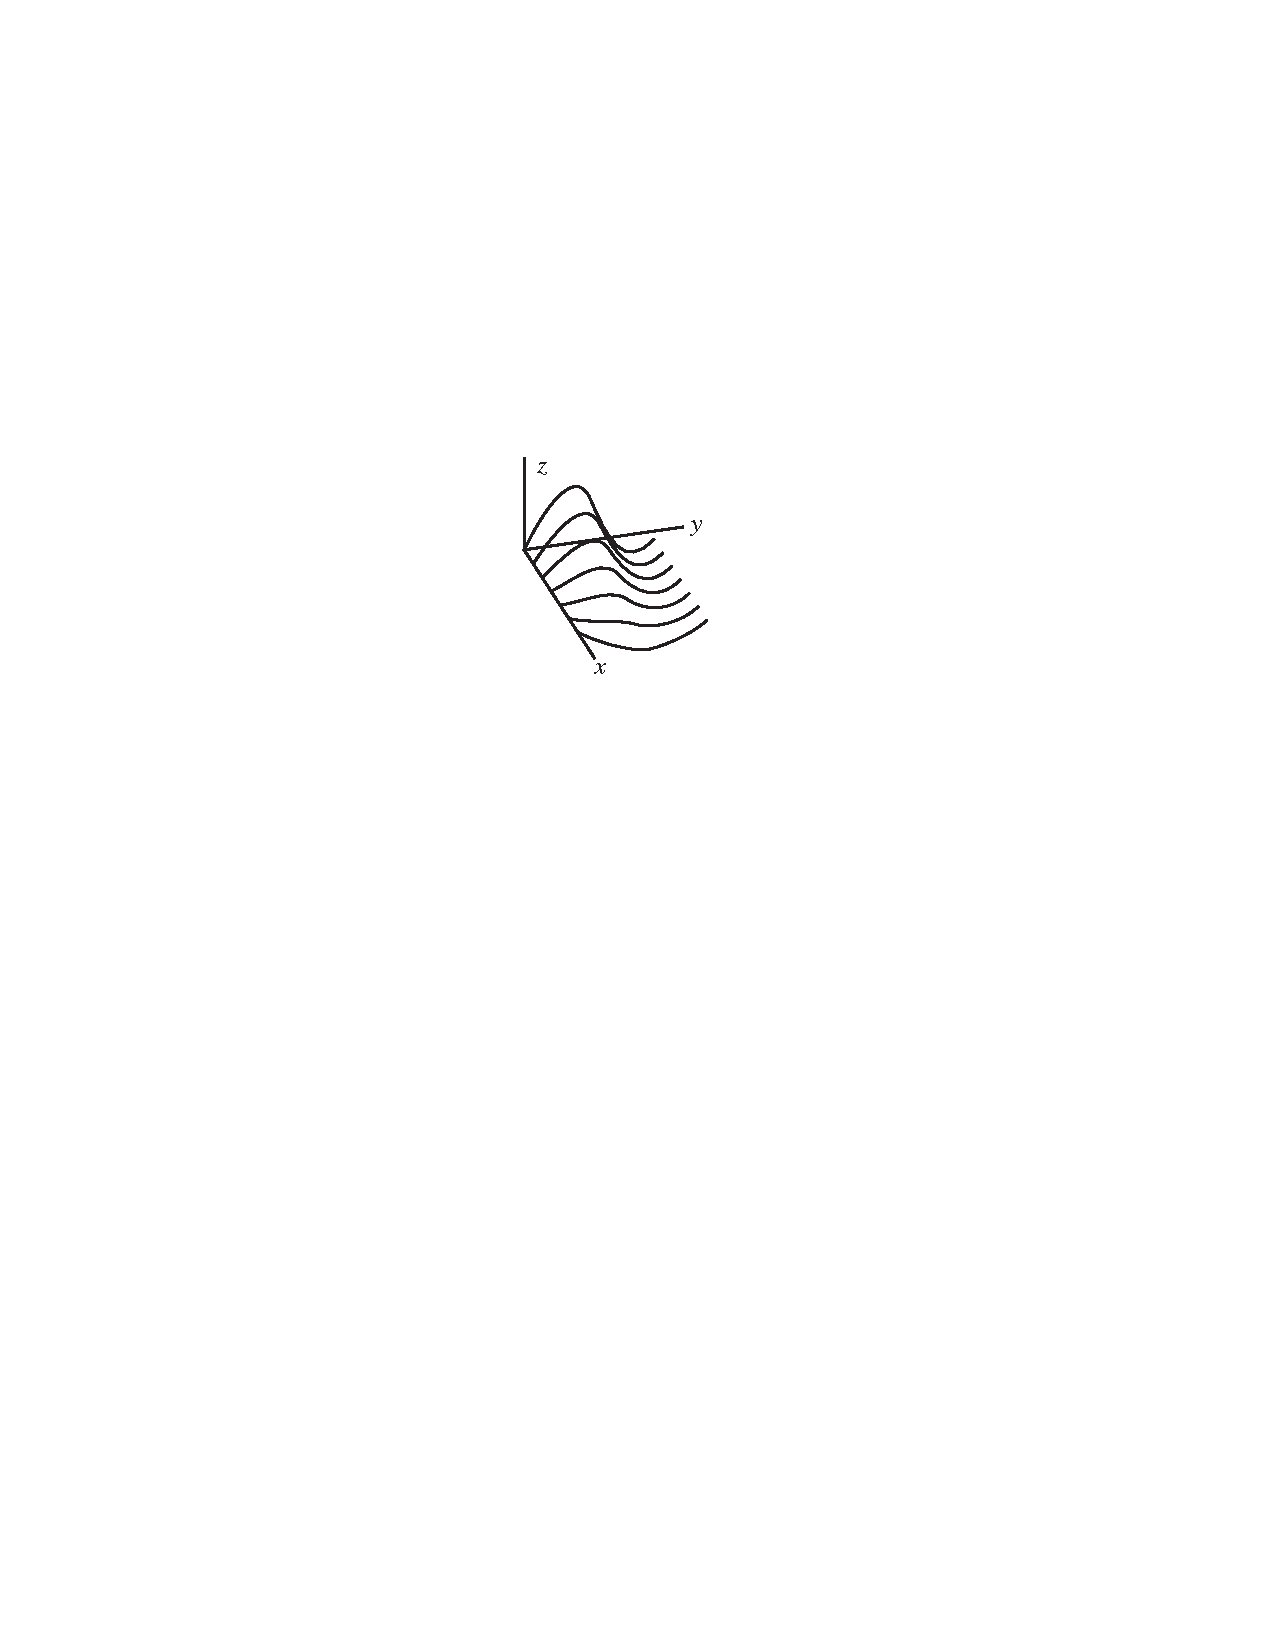
\includegraphics[scale=0.8]{01frozenvariable.pdf} }


\subsection{Moving graphs} 
There is another way of visualizing a function $z=f(x, y)$ of two variables in which we
think of one of the independent variables (e.g.~$y$) as ``time.''  The final picture
is not one static image of a three dimensional surface, but rather a movie of a
graph that is moving around in the $xz$ plane.

If we have a function $z=f(x, y)$, then let us think of $y$ as time, and let us
relabel it as $t$, so that we are looking at the function $z=f(x,t)$. Now at each
moment in time $t$ we can think of $z=f(x,t)$ as a function of one variable $x$ whose
graph we can try to draw, regarding it as a still-image.  Then, as we let time $t$
vary, putting the still images in a sequence, you get a movie of a graph of a
changing function of one variable.

\begin{figure}[b]
  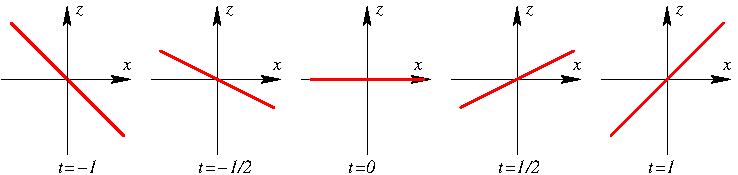
\includegraphics{01saddle-movie.pdf}
  \caption{The saddle movie. It's about a line segment whose slope changes, even
  though it is otherwise stuck to the origin.}
  \label{fig:saddle-movie}
\end{figure}

For instance, if the function is (once again) the saddle surface function $z=xy$,
then we would be considering the function $z=xt$.  At each moment $t$ the graph of
$z=xt$ is a line with slope $t$. Putting these graphs together gives a movie which
begins with a line of rather negative slope;  during the movie the slope increases,
and in the middle of the movie our line has achieved horizontality; finally, the
closing shot presents us with a line with a very positive slope.
Figure~\ref{fig:saddle-movie} shows some stills from the movie.

This interpretation is not very different from the procedure of ``freezing the $y$
variable.'' The only real difference lies in what we do with all the separate graphs
we get after we freeze a variable. In one case we try to piece them together to make
a bigger drawing of a three-dimensional object, in the other we put them together to
make a motion picture.


\section*{Problems} 
\label{sec:graphing-problems-2d3d}
\problemfont 
In the problems in this stage of the course, you will be asked to
``sketch the graph of a function.''  From math 221 you remember that
this meant you had to find minima, maxima, inflection points, and other
features of the graph.  In 234 you will learn to do the same for
functions of two (and more) variables, but for now you should try to
use the method of ``freezing a variable'' or other similar tricks to
get an idea of what the graph of $f$ looks like.

You can use a graphing program (such as \texttt{Grapher.app} on the
Mac, \texttt{GraphCalc} on Windows, or one of the many websites such as
\url{http://www.graphycalc.com/}) to check your answer.

\begin{center}
  \framebox{\parbox{0.4\textwidth}{Note: very often students try to
      fit their drawings into a region the size of a post-it.  In this
      course, whenever you make a drawing, especially if it's a
      three-dimensional drawing, \emph{make it large!}  Use half a
      page for a drawing.  Make sure you have enough paper, try to
      find lots of cheap scrap paper.}}
\end{center}
\begin{multicols}{2}
\problem If we were to drain Lake Mendota, 
as suggested in \S~\ref{sec:01mendotaexample}, would the lake bottom give us the
graph of $d(x, y)$ or of $-d(x,y)$?  (where $d$ is the depth of the lake)?
\answer
$-d(x,y)$.
\endanswer

\problem What are the signs of the coefficients $a$, $b$, and $c$ 
for the linear function whose graph is drawn in Figure~\ref{fig:graph-of-lin-f}?
\answer 
$a<0$, $b>0$, $c>0$.
\endanswer

\problem \itshape About planes and their intersections with the coordinate 
axes.\upshape

\subprob Where does the plane $z=3x-y+6$ intersect the three coordinate axes?
\answer
$x=-2$ for the $x$-axis, $y=6$ for the $y$-axis, $z=6$ for the $z$-axis.
\endanswer

\subprob Find the equation for the plane that intersects 
the $x$-axis at $x=4$, the $y$-axis at $y=2$, and the $z$-axis at $z=3$.
\answer
$z = 3 - \frac34 x - \frac32y$.
\endanswer

\subprob Find the equation for the plane that intersects 
the $x$-axis at $x=a$, the $y$-axis at $y=b$, and the $z$-axis at $z=c$.  (Write
the equation as nice as possible.)
\answer  
$\DS \frac{x}{a} + \frac{y}{b} + \frac{z}{c} = 1$ is a nice symmetric way of
writing the equation.
\endanswer

\problem Find a formula for the distance to the origin of the graph of 
\eqref{eq:linear-function}.
\answer
The distance is $\DS \frac{|c|}{\sqrt{1+a^2+b^2}}$.
\endanswer

\problem 
Classify the following quadratic forms as definite, indefinite, or other, by
completing the square.  Determine the zero set for each of these quadratic forms.

\subprob $f(x, y) = x^2+2y^2$
\answer
This one is already the sum of squares.  We don't have to do anything, and can
immediately conclude that $f(x, y)>0$ for all $(x,y)$ in the plane except the origin,
where $x=y=0$ and $f(x, y) = 0$.
\endanswer

\subprob $Q(x, y) = x^2-y^2$
\answer
The square containing $x$ is already complete (no $xy$ terms) and we can immediately
factor $Q(x, y) = (x-y)(x+y)$.
\endanswer

\subprob $g(x, y) = x^2-4xy + 3y^2$
\answer
We complete the square:
\[
  g(x, y) = (x-2y)^2 - y^2.
\]
We get the difference of two squares, so we can factor the quadratic form:
\[
  g(x, y) = (x-2y - y) (x-2y + y) = (x-3y)(x-y).
\]
\endanswer

\subprob $Q(s,t) = 9s^2-36st + 81t^2$
\answer
This one is positive definite:
\[
  Q 
  = 9\bigl( s^2 - 4st + 9 t^2\bigr)
  = 9\bigl[ (s - 2t)^2 -4t^2 + 9 t^2\bigr]
  = 9\bigl[ (s - 2t)^2 + 5 t^2\bigr]
  =9(s-2t)^2 + 45 t^2.
\]
\endanswer

\subprob $M(\alpha, \beta) = \frac12 \alpha^2 - \alpha\beta+\beta^2$.
\answer
Positive definite:
\[
  M = \frac12\bigl\{\alpha^2- 2\alpha\beta + 2\beta^2\bigr\}
  =\frac12 \bigl\{(\alpha-\beta)^2 + \beta^2\bigr\}.
\]
\endanswer

\subprob $Q(x,y) = xy+y^2$
\answer
This quadratic form has no $x^2$ term.  When that happens you cna immediately factor
the form, because all terms contain $y$:
\[
Q(x,y) = xy+y^2 = (x+y)y.
\]
This form is indefinite.
\endanswer

\subprob $Q(x, y) = x^2+2xy$
\answer
Now this form does have an $x^2$ term, so we \textit{can} complete the square if we
want to \dots but if we look carefully then we see that there's not $y^2$ term.
Because of this we can factor out $x$, and we get
\[
  Q = x^2+2xy = x(x+2y).
\]
The form is indefinite.

What if we don't notice that $y^2$ is missing and just blindly complete the square?
Nothing goes wrong and we get the same answer:
\[
  Q = x^2+2xy = x^2+ 2xy +y^2 - y^2 = (x+y)^2 - y^2 = (x+y - y)(x+y+y) = x(x+2y).
\]
We did work too hard though \verb|:-(|
\endanswer

\problem  For which values of the constant $k$ is the quadratic form
\[
  Q(x, y) = x^2 + 2kxy + y^2
\]
positive definite?
\answer
Complete the square:
\[
  Q=(x+ky)^2 - k^2 y^2 + y^2
   =(x+ky)^2 + (1- k^2) y^2.
\]
If $1-k^2>0$ then we have the sum of two squares.  If $1-k^2<0$, then we can rewrite
$Q$ as the difference of two squares
\[
   Q=(x+ky)^2 - (k^2-1) y^2
   =(x+ky)^2 - \bigl(\sqrt{k^2-1}y\bigr)^2
\]
which is indefinite.  That is all we need to know: we are not actually asked to
factor the form when it is indefinite.  But in case you're wondering, the somewhat
ugly formula is thus:
\[
  Q = \Bigl(x+(k+\sqrt{k^2-1}) y\Bigr) \Bigl(x+(k-\sqrt{k^2-1}) y\Bigr).
\]

The conclusion is that $Q(x,y)$ is positive definite if $-1<k<1$ and indefinite when
$k>1$ or $k<-1$.  In the remaining cases $k=\pm1$ we have
\[
  Q=(x+ky)^2 - k^2 y^2 + y^2
   =(x+ky)^2 + (1- k^2) y^2 = (x\pm y)^2,
\]
i.e.~ the form is a square (it is semidefinite).
\endanswer

\problem\label{prb:some-functions}
Which functions of two variables $z=f(x, y)$ are defined by the
following formulae?
\begin{trivlist}
\item[$\triangleright$] Find draw the domain of each function (the largest domain on
  which the definition would make sense).
\item[$\triangleright$] Try to sketch their graphs.
\item[$\triangleright$] Draw the level sets for each function.
\end{trivlist}

\subprob $z=xy$ 
\answer
The graph is the saddle surface, the function is defined at all $(x,y)$.  The level
set is given by $xy = c$.  If $c\ne 0$ then this set consists of both branches of the
hyperbola $y=\frac{c}{x}$.  If $c=0$ then $xy=0$ is equivalent with $x=0$ or $y=0$,
so the level set is the union of the $x$-and $y$-axes.
\endanswer
\subprob $z-x^2=0$ 
\answer
$z-x^2=0$.
Domain $\R^2$.  Graph is a \emph{parabolic cylinder} and consists of
horizontal lines perpendicular to the $xz$-plane, going through the
parabola $y=x^2$ in that plane.

Level sets: parallel straight lines $x=\pm\sqrt{z}$ if $z>0$,
the $x$ axis if $z=0$, the empty set if $z<0$.
\endanswer
\subprob $z^2-x=0$ 
\answer
$z^2-x=0$.
Implicit function.
At least two functions are defined, namely $z=\pm \sqrt{x}$.
Domain: all points $(x,y)$ with $x\ge 0$.
Graph is \emph{half a parabolic cylinder} and consists of
horizontal lines perpendicular to the $xz$-plane, going through the
parabola $z=\sqrt x$ (or $z=-\sqrt x$, depending on which function
you choose) in that plane.

Level sets (assuming we choose the function $z=+\sqrt{x}$):
the line $x=z^2$ if $z\ge0$, empty set otherwise.
\endanswer
\subprob $z-x^2-y^2=0$
\answer
$z-x^2-y^2=0$.
Domain is the whole plane.
Graph is a paraboloid of revolution, obtained by rotating the
parabola $z=x^2$ in the $xz$-plane around the $z$ axis.

Level sets: circle with radius $\sqrt{z}$ for $z>0$,
the origin for $z=0$ (note: this level set is a point rather than a curve),
empty for $z<0$.
\endanswer
\subprob $z^2-x^2-y^2=0$
\answer
$z^2-x^2-y^2=0$.
Implicit function.  Domain all of $\R^2$.
Possible functions are $z=\pm\sqrt{x^2+y^2}$.
Graph is the cone obtained by rotating the
half line $z=x, x\geq0$ in the $xz$-plane around the $z$ axis
(or the half line $z=-x, x\geq0$, if you chose $z=-\sqrt{x^2+y^2}$.)

Level sets (assuming we choose $z=+\sqrt{x^2+y^2}$):  circle with radius
$z$ when $z>0$, origin when $z=0$, empty when $z<0$.
\endanswer

\subprob $xyz=1$
\answer
$xyz=1$.
Domain the whole plain with the $x$ and $y$-axes removed, i.e.\ all
points $(x, y)$ with $xy\ne0$.
Function is $f(x, y) = \frac{1} {xy}$.
For each $y$ the graph is the hyperbola $z=1/(yx)$ which is just the
standard hyperbola $z=1/x$ stretched vertically by a factor $1/y$.
As $y\to 0$ this factor goes to $\infty$.
\endanswer

\subprob $xy/z^2=1$
\answer
$xy/z^2=1$.
Implicit function.
Domain first and third quadrants (all points with $xy>0$).
Functions $z= \pm \sqrt{xy}$.
Cross sections with planes $y=$constant are half parabolas.

Note: Harder to see, but the surface with equation $xy=z^2$ is in fact
the cone obtained by rotating the $x$-axis around the line
$x=y$ in the $xy$-plane.
\endanswer

\subprob $x+y+z^2=0$

\subprob $x+y+z^2=1$

\problem\label{prb:polar-angle-formula} 
The following expressions are all equal to the polar angle $\theta$ in some region of
the $xy$-plane.  Explain why the expression gives $\theta$, and identify in which
region this holds.

\subprob $\DS \theta = \arctan \frac{y}{x}$
\answer
$x>0$.  This one is in the text.
\endanswer

\subprob $\DS \theta = \pi+\arctan \frac{y}{x}$
\answer
$x<0$.
\endanswer

\subprob $\DS \theta = 2\pi+\arctan \frac{y}{x}$
\answer
$x>0$.  This is the same region as in part (a):  remember that the polar angle is
only determined up to a multiple of $2\pi$.
\endanswer

\subprob $\DS \theta = \frac\pi2 - \arctan \frac{x}{y}$
\answer
In the upper half plane, $y>0$.
\endanswer

\subprob $\theta=\arcsin \frac{y}{\sqrt{x^2+y^2}}$.
\answer
In the whole plane, except the origin, and the negative $x$-axis.  This formula for
the polar angle $\theta$ clearly is valid in a larger region than the other formulas,
but it does not look half as nice.
\endanswer


\problem {\itshape``The level set is always a curve\dots'' --- not!}\\ 
If $d(x, y)$ is the depth function of Lake Mendota (see
\S\ref{sec:01mendotaexample}), then what are the level sets $d^{-1}(c)$
for $c=0$, $c=+24$ and for $c=-24$ (meters)?  What is the level
set $d^{-1}(400)$ (meter)?
\answer 
The level set for $c=-24$ is the empty set, since it consists of all points on
the lake surface where the lake is $-24$ meters deep--i.e.~where the water
reaches $24$meters {\bfseries\itshape above} the lake.    

Similarly, the level set for $c=+400$ is also empty since the lake is not that
deep anywhere.

The level set $d^{-1}(0)$ consists of those points where the lake is $0$meters
deep.  This is exactly the shore line.

The level set $d^{-1}(24)$ consists of all points on the lake surface where the
lake is exactly $24$meters deep.  Form the map it looks like this happens on two
separate curves near the center of the lake.
\endanswer



\problem Describe and explain the relation between the graph of the 
function $y=g(x)$ of one variable, and the corresponding function
$f(x, y) = g\bigl( \sqrt{x^2+y^2} \bigr)$ of two variables.

What do the level sets of $f(x, y)$ look like?

For instance, if $g(x) = x$, then $f(x, y) = \sqrt{x^2+y^2}$: what is
the relation between the graphs of $g$ and $f$?
\answer
See \S~\ref{sec:functions-in-PC}.
\endanswer


\problem Find the largest domain on which 
the following functions of two (or occasionally three) variables can be defined:

\subprob  $f(x, y) = \sqrt{9-x^2}+\sqrt{y^2-4}$
\answer
The two rectangular strips $-3\leq x\leq3, 2\leq y<\infty$ and
$-3\leq x\leq3, -\infty<y\leq-2$.
\endanswer

\subprob  $f(x, y) = \arcsin(x^2+y^2-2)$
\answer
By definition $\arcsin(x)$ is only defined if $-1\leq x\leq1$.
For $\arcsin(x^2+y^2-2)$ to be defined, we must therefore have
$-1\leq x^2+y^2-2 \leq 1$, i.e.\ $1\leq x^2+y^2 \leq 3$.

The domain of this function is
the ring-shaped region between the circles with radii $1$ and
$\sqrt{3}$, both centered at the origin.
Circles are included in the domain.
\endanswer

\subprob  $f(x, y) = \sqrt{x}\;\cdot\;\sqrt{y}$
\answer
The way this function is written both $\sqrt x$ and $\sqrt y$ must be defined,
so the domain consists off all $(x,y)$ with $x\geq0$ and $y\geq0$.
\endanswer

\subprob  $f(x, y) = \sqrt{xy}$
\answer
$\sqrt{xy}$ must exist, which happens for all $(x,y)$ in the first
and third quadrants (axes included.)
\endanswer

\subprob  $f(x, y, z) = 1/\sqrt{xyz}$

\subprob  $f(x, y) = \sqrt{16-x^2-4y^2}$
\answer
The region in the plane given by $x^2+4y^2\leq16$, which is the region
enclosed by an ellipse with
major axis of length 4, along the $x$ axis, and minor axis of length
2 along the $y$-axis.  The ellipse is included.
\endanswer

\problem\label{prb:cone-or-paraboloid}
Here are two sets of level curves with levels $z=0.2, 0.4, 0.6, 0.8,
1.0, 1.2,  1.4$.  One is for a function whose graph is a cone
($z=\sqrt{x^2+y^2}$), the other is for a paraboloid ($z=x^2+y^2$).
Which is which? Explain.
\answer
The level sets of the function whose graph is a cone are equally spaced circles
(the level set at level $c$ is a circle with radius $c$).  Hence the one on the
right corresponds to the cone, and
the one on the left corresponds to the paraboloid.
\endanswer
\begin{center}
  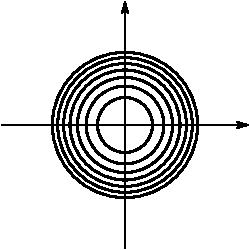
\includegraphics[scale=0.7]{01paraboloidLevels.pdf}
  \quad
  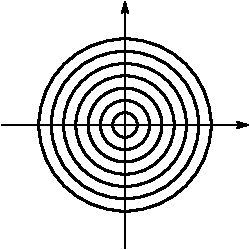
\includegraphics[scale=0.7]{01coneLevels.pdf}
\end{center}

\problem\label{prb:distance-to-square-level-sets}
\carefulnow~
Let $Q$ be the square in the plane consisting of all points $(x,y)$
with $|x|\le1$, $|y|\le1$.  This problem is about the so-called
\emph{distance function} to $Q$.  This function is defined as
follows:  $f(x, y)$ is the distance from the point $(x,y)$ to the
point in $Q$ nearest to $(x,y)$.

\subprob Which point in $Q$ is nearest to $(0, \frac12)$?  Which is
closest to $(0, 2)$?  Which is closest to $(3,4)$?
\answer
$(0, \frac{1} {2})$ is in the square $Q$, so it is the point closest to
$(0, \frac{1} {2})$.\\
The point $(0,1)$ on the top edge of the square is closest to $(0,2)$.\\
The corner point $(1,1)$ is closest to $(3,4)$.
\endanswer

\subprob Compute $f(0, \frac12)$, $f(0,2)$ and $f(3, 4))$.
\answer
$f(0, \frac12) =0 $;
$f(0,2)=1$ and $f(3, 4))=\sqrt{2^2+3^2}=\sqrt{13}$.
\endanswer

\subprob What is the zero set of $f$?
\answer
The zero set of $f$ is the square $Q$.
\endanswer

\subprob Draw the level sets of $f$ at levels $-1$, 1, 2, and 3.  Describe
the general level set $f(x, y) = c$ where $c$ is an arbitrary number.
\answer
The level set at level $-1$ is empty.  The others are ``rounded
rectangles,'' see this drawing, in which the square is grey, the dashed
lines are given by $x=\pm1$ or $y=\pm1$.
\begin{center}
    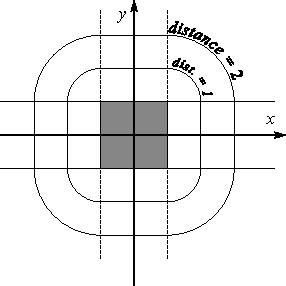
\includegraphics{01distancetosquare.pdf}
\end{center}
\endanswer

\subprob Give a formula for $f(x, y)$.  (It turns out to be too hard to
capture the distance function in one formula.  You will have to split the
plane into different regions and describe $f(x,y)$ by different formulas,
according to which region $(x,y)$ belongs to.)
\answer
The lines $x=\pm1$ and $y=\pm1$ divide the plane into nine regions.
On each region the function is given by a different formula.
Here they are:
\begin{tabbing}
\=$\boldmath{f(x, y)}$ \=\`\textbf{ if } \ldots \\
\>$0$  \>\` $(x, y)$ in $Q$\\
\>$x-1$ \>\` $x\geq1, |y|\leq 1$\\
\>$y-1$ \>\` $|x|\leq 1, y\geq1$\\
\>$-x-1$ \>\` $x\le-1, |y|\leq 1$\\
\>$-y-1$ \>\` $|x|\leq 1, y\le-1$\\
\>$\sqrt{(x-1)^2+(y-1)^2}$ \>\` $x\ge1$ and $y\ge1$\\
\>$\sqrt{(x-1)^2+(y+1)^2}$ \>\` $x\ge1$ and $y\le-1$\\
\>$\sqrt{(x+1)^2+(y-1)^2}$ \>\` $x\le-1$ and $y\ge1$\\
\>$\sqrt{(x+1)^2+(y+1)^2}$ \>\` $x\le-1$ \& $y\le-1$\\
\end{tabbing}
\endanswer

\problem  Describe the ``movie'' that goes with each of the following 
functions.

\subprob $f(x, t) = x\sin t$
\answer
At time $t$ we have a line through the origin with slope $\sin t$.
As time progresses this lines turns up and down, and up and down,  etc.
\endanswer
\subprob $f(x, t) = x\sin 2t$
\answer
Same as previous problem, but twice as fast.
\endanswer

\subprob $f(x, t) = t\sin x$
\answer
At all times one sees the graph of $y=\sin x$ stretched vertically by a factor $t$.
\endanswer

\subprob $f(x, t) = 2t \sin x$
\answer
Same as previous problem, but twice as fast.
\endanswer
\subprob $f(x, t) = t\sin 2x$
\answer
The graph of $y=\sin 2x$ stretched vertically by a factor $t$.
\endanswer

\subprob $f(x, t) = (x-t)^2$
\answer
Parabola with its minimum on the $x$-axis at $x=t$.
So we see the parabola $y=x^2$ translating from the left to the right
with constant speed 1.
\endanswer

\subprob $f(x, t) = (x-\sin t)^2$
\answer
Parabola with its minimum on the $x$-axis at $x=\sin t$.
So we see the parabola $y=x^2$ translating back and forth horizontally
every $2\pi$ time units.
\endanswer

\subprob $f(x, t) = (x-t^2)^2$

\subprob $f(x, t) = \dfrac{t^2}{1+x^2}$

\subprob $f(x, t) = \dfrac{1}{(1+x^2) (1+t^2)}$
\answer
At time $t$ we see Agnesi's witch, i.e. the graph $y= a/(1+x^2)$
with amplitude $a=1/(1+t^2)$.  Thus we see a bump whcich starts out small
 at $t=-\infty$, grows to its maximal size at time $t=0$, and then decays
again, until it vanishes at $t=+\infty$.
\endanswer

\problem Describe the movie that goes with the function
\[
  f(x, t) = \arctan \frac xt,
\]
for $t>0$.  The function is not defined at $t=0$, but can you describe the limit
of this function as $t\to0$?  (Hint: the sign of $x$ matters).


\problem \label{prb:01traveling-waves}
If $y=g(x)$ is any function of one variable, then a function of the
form $f(x, t) = g(x-ct)$ is often called a \emph{traveling wave} with
wave speed $c$ and profile $g$.  Let $g$ be any non constant
function of your choice and describe the movie presented by the
function $f(x, t) = g(x-ct)$ (can't choose?  Then try ``Agnesi's
witch'' $g(x) = \frac{1}{1+x^2}$.)

The number $c$ is called the wave speed.  If $c>0$ is the motion to
the left or to the right? Explain.
\answer
The graph of $y=g(x-a)$ is obtained from the graph of $y=g(x)$ by
translating the graph of $y=g(x)$ by $a$ units to the right.

Hence the graph of $g(x-ct)$ is the graph of $g(x)$ translated by $ct$
units to the right.  As time changes the graph of $g(x-ct)$ therefore
moves with velocity $c$ to the right.
\endanswer


\problem If $y=g(x)$ is any function of one variable, then a function 
of the form
\[
  f(x, t) = \cos(\omega t) g(x)
\]
is often called a \emph{standing wave.}
Let $g$ be any non constant function of your choice and describe the
movie presented by the function $f(x, t) = \cos(\omega t)g(x)$
(can't choose?  Then try ``Agnesi's witch''  $g(x) = \frac{1}{1+x^2}$
again, or for this example, try $g(x) = \sin x$.)

The number $\frac\omega{2\pi}$ is called the frequency of the standing
wave.  The function $g(x)$ is called its profile.  How long does it
take before the standing wave returns to its original position, i.e.\
what is the smallest $T>0$ for which $f(x, T) = f(x, 0)$ for all $x$?
Explain.
\answer
If you know the graph of a function $y=g(x)$, then you get
the graph of $y=cg(x)$ by stretching the graph of $g$ vertically by
a factor $c$ (here $c$ is a constant.)
If you allow this constant to depend on time, e.g.\ as in this
problem by setting $c=\cos(\omega t)$, then the ``movie'' you get is of a
version of the graph of $g$ which is growing and shrinking vertically.

\begin{center}
    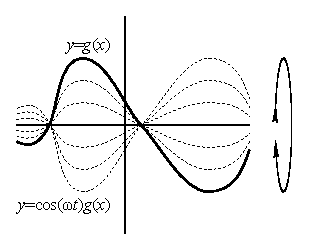
\includegraphics{01standingwave.pdf}
\end{center}
\endanswer
\end{multicols}
\noproblemfont


%%% Local Variables: 
%%% mode: latex
%%% TeX-master: "free234"
%%% End: 
